%%%%%%%%%%%%%%%%%%%%%%%%%%%%%%%%%%%%%%%%%
% baposter Landscape Poster
% LaTeX Template
% Version 1.0 (11/06/13)
%
% baposter Class Created by:
% Brian Amberg (baposter@brian-amberg.de)
%
% This template has been downloaded from:
% http://www.LaTeXTemplates.com
%
% License:
% CC BY-NC-SA 3.0 (http://creativecommons.org/licenses/by-nc-sa/3.0/)
%
%%%%%%%%%%%%%%%%%%%%%%%%%%%%%%%%%%%%%%%%%

%----------------------------------------------------------------------------------------
%	PACKAGES AND OTHER DOCUMENT CONFIGURATIONS
%----------------------------------------------------------------------------------------

\documentclass[landscape,a0paper,fontscale=0.35]{baposter} % Adjust the font scale/size here

\usepackage{graphicx} % Required for including images
\graphicspath{{figures/}} % Directory in which figures are stored

\usepackage{amsmath} % For typesetting math
\usepackage{amssymb} % Adds new symbols to be used in math mode

\usepackage{booktabs} % Top and bottom rules for tables
\usepackage{enumitem} % Used to reduce itemize/enumerate spacing
\usepackage{palatino} % Use the Palatino font
\usepackage[font=small,labelfont=bf]{caption} % Required for specifying captions to tables and figures

\usepackage{multicol} % Required for multiple columns
\setlength{\columnsep}{1.5em} % Slightly increase the space between columns
\setlength{\columnseprule}{0mm} % No horizontal rule between columns

\usepackage{tikz} % Required for flow chart
\usetikzlibrary{shapes,arrows} % Tikz libraries required for the flow chart in the template


\newcommand{\compresslist}{ % Define a command to reduce spacing within itemize/enumerate environments, this is used right after \begin{itemize} or \begin{enumerate}
\setlength{\itemsep}{1pt}
\setlength{\parskip}{0pt}
\setlength{\parsep}{0pt}

\setlength{\paperwidth}{36in}
\setlength{\paperheight}{24in}
}

\definecolor{lightblue}{rgb}{0.145,0.6666,1} % Defines the color used for content box headers

\begin{document}

\begin{poster}
{
headerborder=closed, % Adds a border around the header of content boxes
colspacing=1em, % Column spacing
bgColorOne=white, % Background color for the gradient on the left side of the poster
bgColorTwo=white, % Background color for the gradient on the right side of the poster
borderColor=lightblue, % Border color
headerColorOne=black, % Background color for the header in the content boxes (left side)
headerColorTwo=lightblue, % Background color for the header in the content boxes (right side)
headerFontColor=white, % Text color for the header text in the content boxes
boxColorOne=white, % Background color of the content boxes
textborder=roundedleft, % Format of the border around content boxes, can be: none, bars, coils, triangles, rectangle, rounded, roundedsmall, roundedright or faded
eyecatcher=true, % Set to false for ignoring the left logo in the title and move the title left
headerheight=0.1\textheight, % Height of the header
headershape=roundedright, % Specify the rounded corner in the content box headers, can be: rectangle, small-rounded, roundedright, roundedleft or rounded
headerfont=\Large\bf\textsc, % Large, bold and sans serif font in the headers of content boxes
%textfont={\setlength{\parindent}{1.5em}}, % Uncomment for paragraph indentation
linewidth=2pt % Width of the border lines around content boxes
}
%----------------------------------------------------------------------------------------
%	TITLE SECTION 
%----------------------------------------------------------------------------------------
%
{
\includegraphics[height=5em]{ONR_logo.png}} % First university/lab logo on the left
{\bf\textsc{Follow The Leader}\vspace{0.1em}} % Poster title
{\textsc{ Andy Vo (CSE), Hugh Fong (CpE), Lawrence Dizon (CSE), David Phan (CpE)  \hspace{15pt} Mahdi Maaref, Department of Electrical Engineering and Computer Science} } % Author names and institution
{
\includegraphics[height=5em]{UCI_Logo.png}} % Second university/lab logo on the right

%----------------------------------------------------------------------------------------
%	Project Goal
%----------------------------------------------------------------------------------------

\headerbox{Project Goal}{name=objectives,column=0,row=0}{

In our project, we focus on having an autonomous follower drone to follow a primary leader drone. The project would help improve military technology by exploring ways for a single drone to communicate or control multiple autonomous drones.

%\begin{enumerate}\compresslist

%\end{enumerate}

\vspace{0.3em} % When there are two boxes, some whitespace may need to be added if the one on the right has more content
}

%----------------------------------------------------------------------------------------
%	Background
%----------------------------------------------------------------------------------------

\headerbox{Background}{name=introduction,column=1,row=0,bottomaligned=objectives}{

Drones are currently used in military surveillance. Although drones are a useful piece of technology, there is a need for better drone coordination; drone coordination still has room for improvement, which will greatly improve surveillance operations. 
}

%----------------------------------------------------------------------------------------
%	Progress
%----------------------------------------------------------------------------------------

\headerbox{Progress}{name=results,column=2,span=2,row=0}{

\begin{multicols}{2}
\vspace{1em}
\begin{center}
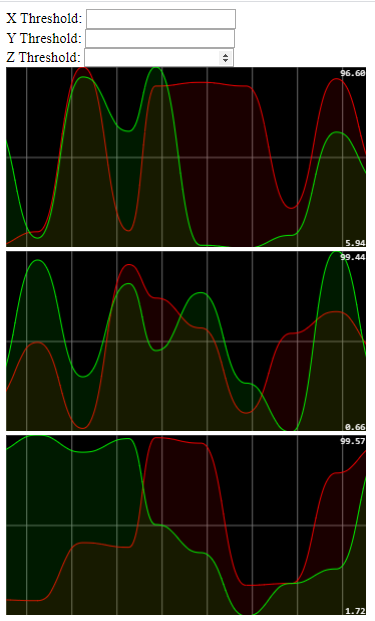
\includegraphics[scale=0.3]{GUI}
\end{center}

The GUI has been implemented so that the user can change the threshold difference between the follower drone and the leader drone.  Real-time graphs are created so that both of the GPS locations of the leader drone and the follower drone are displayed; each graph represents the latitude, longitude, and elevation of each drone. 
\end{multicols}

%------------------------------------------------

\begin{multicols}{2}
\vspace{1em}

We have implemented PID controllers for drone movement. PID stands for proportional, integral and derivative. The controllers will
continuously calculate the error by subtracting the set value with the actual value and its job is to reduce the error to be close to zero.
This allows the drone to fly autonomously and to match the distance thresholds as close as possible.

\begin{center}
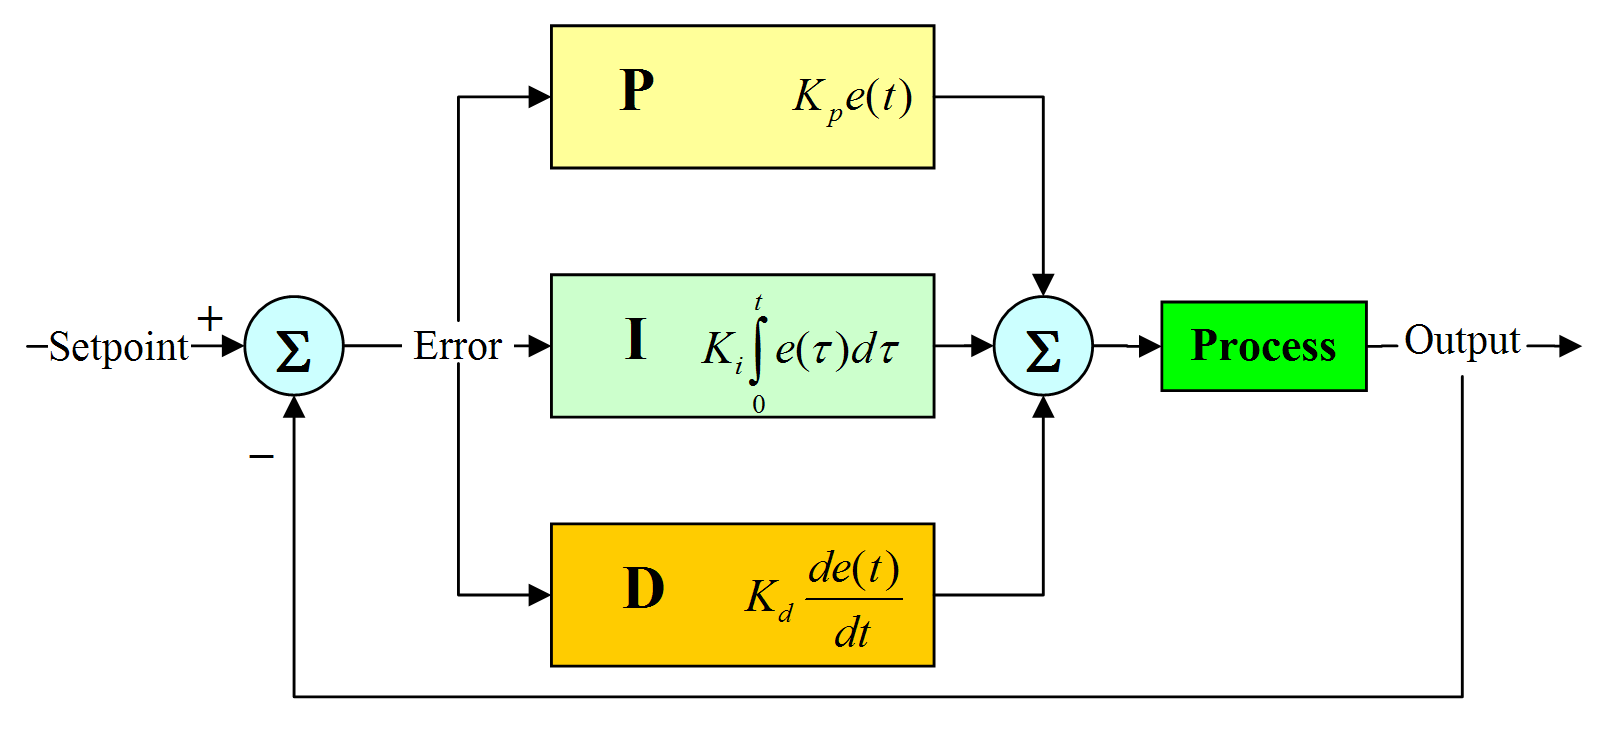
\includegraphics[width=70mm]{PID_Image}
\end{center}

\end{multicols}
}

%----------------------------------------------------------------------------------------
%	REFERENCES
%----------------------------------------------------------------------------------------
\footnotesize\headerbox{References}{name=references,column=0,above=bottom}{
\begin{itemize}\compresslist
\item [1] P. Bouman, et al. Dynamic Programming Approaches for the Traveling Salesman Problem with Drone. Networks, vol. 72, no. 4, 2018, pp. 528–542.
\item [2] L. Mottola et al. Team-Level Programming of Drone Sensor Networks. Proceedings of the 12th ACM Conference on Embedded Network Sensor Systems - SenSys '14, 2014. 
\end{itemize}
}

%----------------------------------------------------------------------------------------
%	FUTURE RESEARCH
%----------------------------------------------------------------------------------------

\headerbox{Future Research}{name=futureresearch,column=1,span=2,aligned=references,above=bottom}{ % This block is as tall as the references block

\begin{multicols}{2}
Object detection through a camera attached to the drone will allow the drone to avoid obstacles while flying towards the GPS coordinates of the leader.

The drone's ability to autonomously return back to the base station will also be impilemented. The drone will either backtrack using previous GPS coordinates, or calculate the shortest distance and fly straight to the base station. 
\end{multicols}
}

%----------------------------------------------------------------------------------------
%	CONTACT INFORMATION
%----------------------------------------------------------------------------------------

\headerbox{Contact Information}{name=contact,column=3,aligned=references,above=bottom}{ % This block is as tall as the references block

\begin{description}\compresslist
\item Andy Vo - andytv1@uci.edu 
\item Hugh Fong - hyfong@uci.edu
\item Lawrence Dizon - dizonl@uci.edu
\item David Phan - ddphan2@uci.edu
\end{description}
}

%----------------------------------------------------------------------------------------
% 	Challenges
%----------------------------------------------------------------------------------------

\linespread{1.5}\headerbox{Challenges}{name=conclusion,column=2,span=2,row=0,below=results,above=references}{

%------------------------------------------------
In order to send data to the follower drone from the leader drone, GPS modules attached to a Raspberry Pi will be used to communicate to the base station, where the flight path for the follower drone will be created.GPS data was only obtainable from a single drone at a time due to the base station being unable to connect to two different wifi connections. Another issue was the relaying of data between the GUI and the base station. Both of these were written in incompatible programming languages, thus raising a problem. A framework to integrate the GUI and base station was needed, and was a challenge. The control flow of NodeJS was unfamiliar to us, causing unexpected behaviors that we did not expect. 

}

%----------------------------------------------------------------------------------------
%	MATERIALS AND METHODS
%----------------------------------------------------------------------------------------

\linespread{1.1}\headerbox{Materials \& Methods}{name=method,column=0,below=objectives,bottomaligned=conclusion}{ % This block's bottom aligns with the bottom of the conclusion block
Computations to obtain desired heading: 
\\
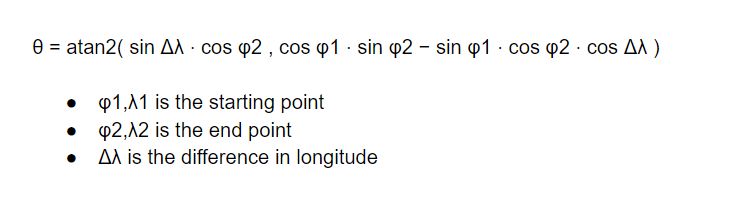
\includegraphics[scale=0.27]{Equation}
%\begin{equation}
%E = mc^{2}
%\label{eqn:Einstein}
%\end{equation}
We enabled and calibrate the drone's magnetometer then obtain the drone's magnetic heading as well
as current coordinates. Next, we calculate the desired heading which is the direction of the leader drone
relative to the follower drone. The drone then rotates until it achieves the desired heading and then
flies forward. The drone also increases its elevation until it is within a certain threshold of the leader drone.
\\
Drone connection will be established via a router. The router will allow a connection between a Raspberry Pi that will be attached to our Leader drone, the autonomous follower drone, and a laptop that will act as our base station. The Raspberry Pi will collect GPS coordinates of the Leader drone and perform the computation needed to alter the flight path of the follower drone. The flight controller is implemented in NodeJS.
}

%----------------------------------------------------------------------------------------
%	Conclusion
%----------------------------------------------------------------------------------------

\linespread{1.5}\headerbox{Conclusion}{name=results2,column=1,below=objectives,bottomaligned=conclusion}{ % This block's bottom aligns with the bottom of the conclusion block

The Raspberry Pi (attached to leader drone) will be used for computing the flight control for the follower drone.The follower drone receives NodeJS flight control commands to correct its path to follow the leader. The raspberry PI also sends data to the laptop so that it can display it in the GUI. 
\\
\\
\\
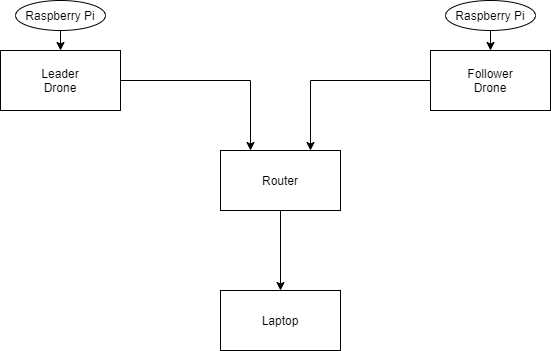
\includegraphics[scale=0.35]{New_Drone_Connection_Diagram}

}

%----------------------------------------------------------------------------------------

\end{poster}

\end{document}